\documentclass[a4paper]{article}
\usepackage{graphicx}
\usepackage{wrapfig}
\usepackage{caption}
\usepackage{subcaption}
\usepackage{amsfonts} 


\title{Merge Sort}
\author{Yarne Ramakers}
\date{\today}

\begin{document}

%\maketitle - had to comment as it took up too much space
\begin{center}
  Merge Sort \\
  Yarne Ramakers \\
  \today \\
\end{center}

\begin{figure}[h]
  \begin{subfigure}{0.3\textwidth}
    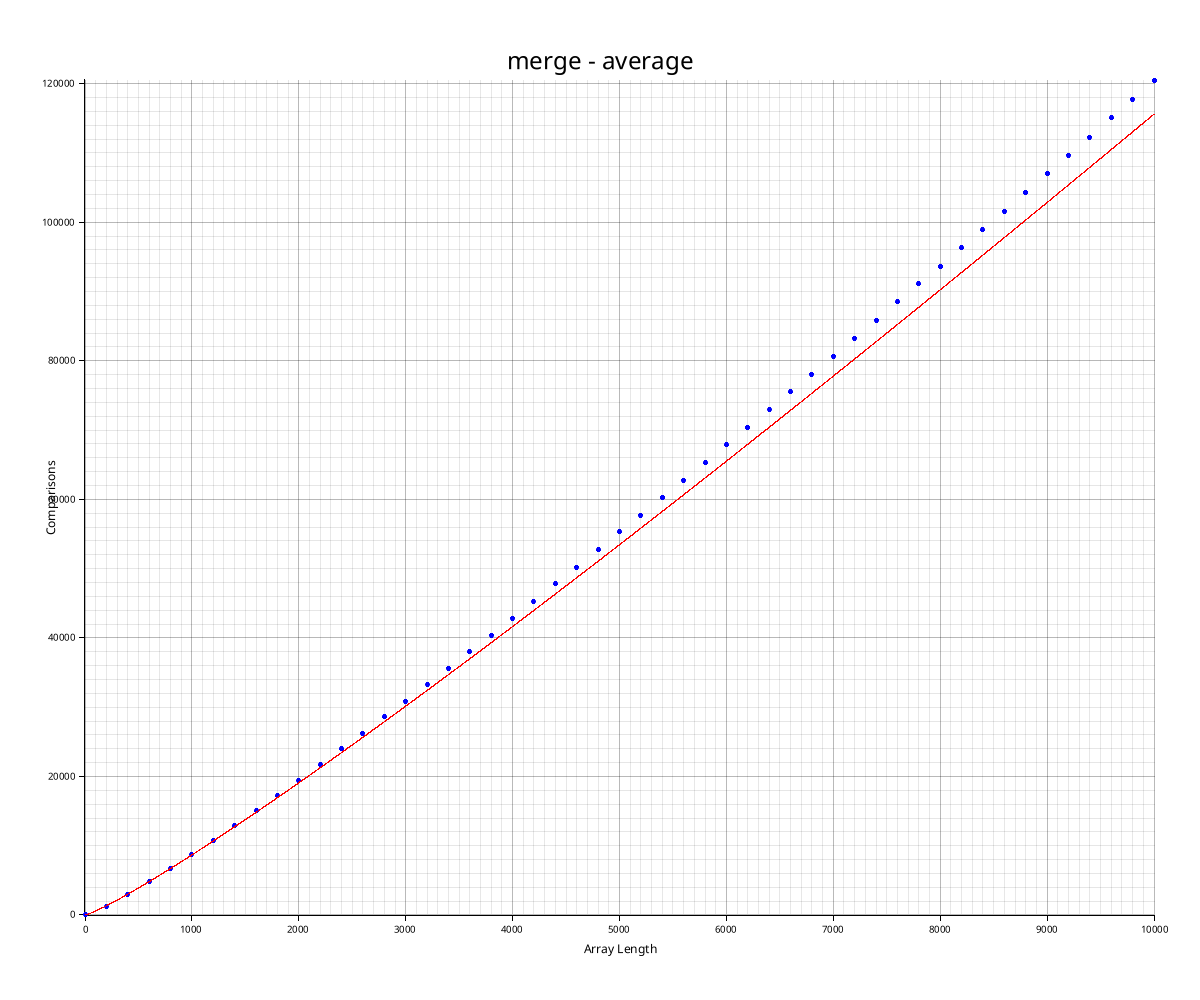
\includegraphics[width=\textwidth]{../plots/merge-average.png}
    \caption{Average case}
    \label{fig:merge-avg}
  \end{subfigure}
  \begin{subfigure}[b]{0.3\textwidth}
    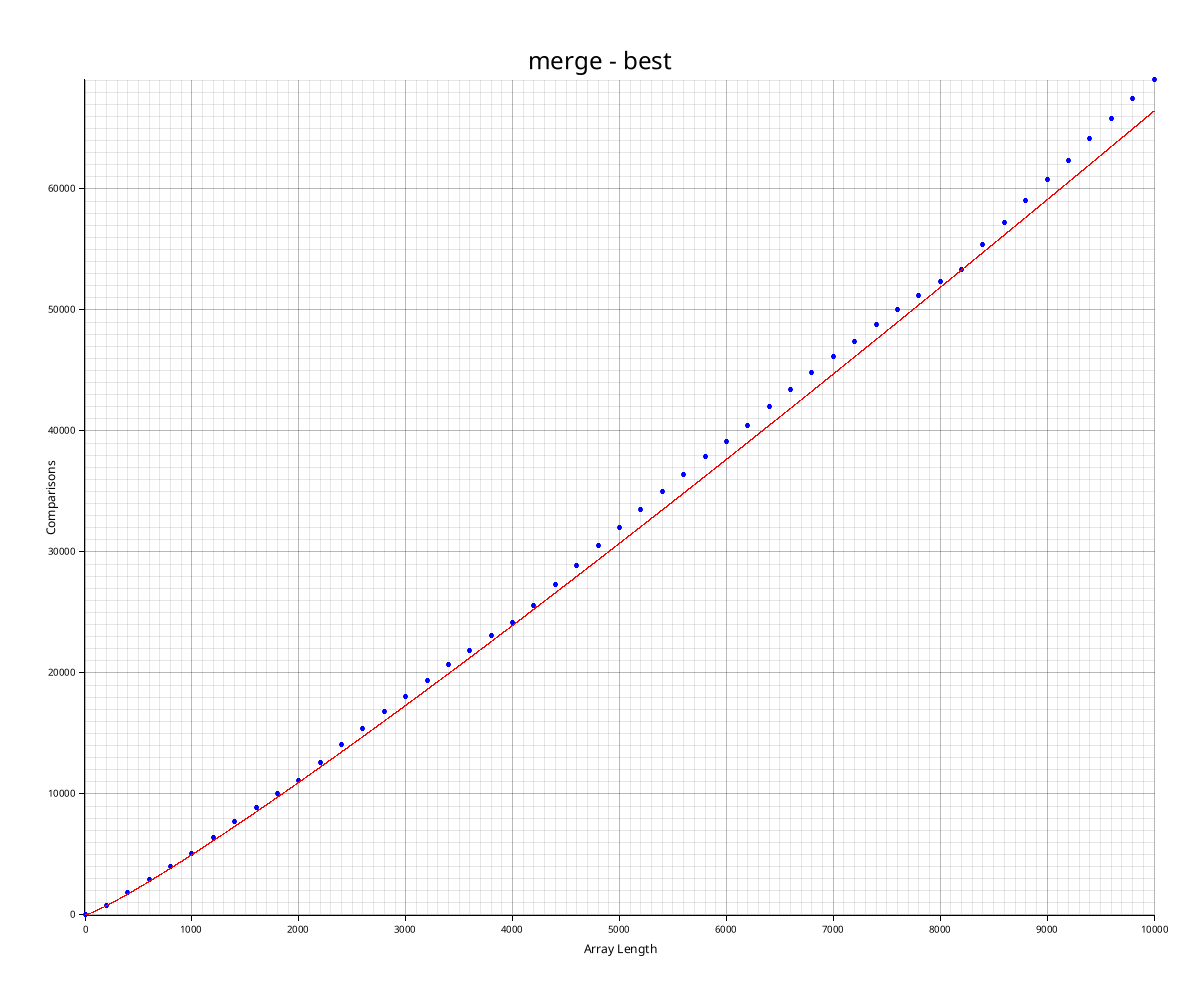
\includegraphics[width=\textwidth]{../plots/merge-best.png}
    \caption{Best case}
    \label{fig:merge-best}
  \end{subfigure}
  \begin{subfigure}[b]{0.3\textwidth}
    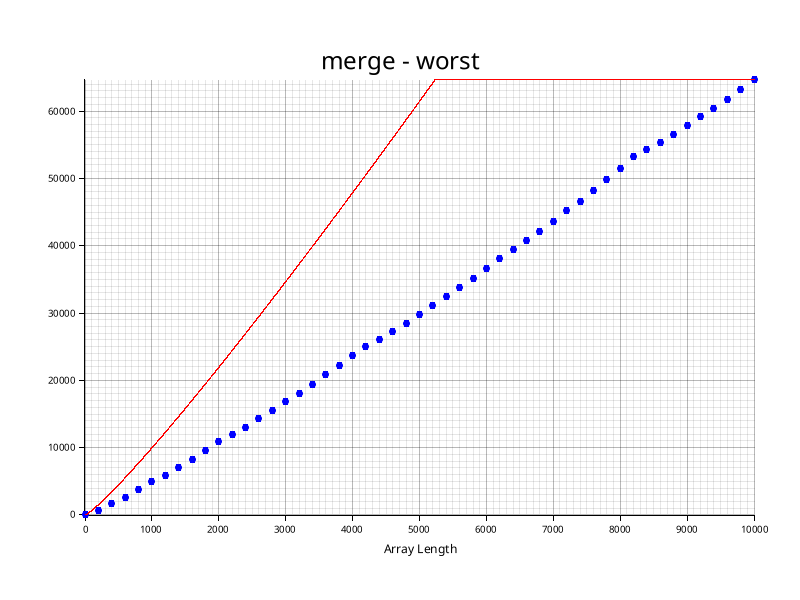
\includegraphics[width=\textwidth]{../plots/merge-worst.png}
    \caption{Worst case}
    \label{fig:merge-worst}
  \end{subfigure}
\end{figure}

\section{Introductie}
% Introduction to merge sort and its importance.
Merge sort is een sorteeralgoritme dat gebruik maakt van het verdeel en heers principe.

\section{Bevindingen}
% Discuss the results of the experiments.
Mijn experimentele bevinding vertonen sterke overeenkomsten met het theoretische model van merge sort.
De grafieken \ref{fig:merge-best} en \ref{fig:merge-worst} tonen de theoretische complexiteit van merge sort in best case en worst case respectievelijk.
De rode lijn toont de theoretische complexiteit van merge sort, namelijk $\sim \frac{1}{2} n \log n$ en $\sim n \log n$ respectievelijk.
De blauwe punten tonen de gemeten vergelijkingen over lijsten voor verschillende lengte $n$. 
Deze $n$ is gekozen tussen 0 en 10 000 met een stapgrootte van 200, per $n$ zijn er ook 10 metingen gebeurd.
\par
We merken wel op dat de gemeten vergelijkingen afwijken van de theoretische complexiteit, naarmate $n$ groter wordt.
Dit komt omdat de overhead van het meten van de complexiteit een grotere invloed heeft op de gemeten complexiteit.
Wat ook opmerkelijk is, is dat de gemeten complexiteit voor lijsten van lengte $n=2^k$ met $k \in \mathbb{N}$ gelijk is aan de theoretische complexiteit.
\par
De grafiek \ref{fig:merge-avg} toont de theoretische complexiteit van merge sort in het gemiddelde geval.
We weten dat dit gedrag tussen $\sim \frac{1}{2} n \log n$ en $\sim n \log n$ zal liggen. Dit zal dus gelijk zijn aan $\sim cn \log n$. Met $\frac{1}{2}<c<1$.
Ik heb geprobeerd deze $c$ te bepalen door de gemeten complexiteit $+n-1$ te delen door $n \log n$. Deze waarde varrieert echter heel erg.
Bij kleinere $n$ lag deze $c$ vaak rond de $0.84-0.85$ terwijl bij grotere $n$ deze waarde eerder rond de $0.88-0.90$ lag.
Ik heb dan besloten om de mediaan van deze metingen te nemen en vond dan dat $c=0.87$. In grafiek \ref{fig:merge-avg} stelt de rode lijn de theoretische complexiteit voor, namelijk $\sim 0.87n \log n$.
Hier valt inderdaad op te merken dat voor kleine $n$ de gemeten complexiteit eerder onder deze curve ligt, terwijl lijsten met grote $n$ eerder naar boven zullen afwijken van deze curve.
\par
Dit wil zeggen dat de gemeten complexiteit van merge sort in het gemiddelde geval gelijk is aan $\sim 0.87n \log n$.
Het gemiddelde geval zal dus eerder naderen naar de theoretische complexiteit van merge sort in het slechtste geval.

\end{document}